\documentclass{exam}
%==================================================================================
% I. Preambulo
%==================================================================================
%----------------------------------------------------------------------------------
% 1.Paquetes
%----------------------------------------------------------------------------------
\usepackage[spanish]{babel}			% escribir en espanol
\usepackage[utf8]{inputenc}	    % escribir en espanol
\usepackage{amsmath}				% ecuaciones y demases
\usepackage{amsthm}					% ecuaciones y demases
\usepackage{amssymb}				% ecuaciones y demases
\usepackage{graphicx}		        % graficos
\usepackage{float}					% manejar la ubicacion de graficos
\usepackage{verbatim}				% Para escribir codigos
\usepackage{url}					% Para escribir direcciones web
%\usepackage{subfig}					% Para poner varias figuras en el mismo marco
\usepackage{psfrag}					% Para hacer reemplazos en las figuras
\usepackage{multicol}
\usepackage{multirow}
\usepackage{bigstrut}
\usepackage{color}
\usepackage{tabularx}               % tablas
\usepackage{amstext}
\usepackage[utf8]{inputenc}
\usepackage{graphicx}
\usepackage{adjustbox}
\usepackage{gensymb}
\usepackage{enumerate}
\usepackage{enumitem}        % Enumerar elementos
\usepackage{enumitem}[a)]
\usepackage{enumerate}[a)]
\usepackage{enumerate}[a.]
\spanishdecimal{.}

%----------------------------------------------------------------------------------
% 2.Estilo de la pagina
%----------------------------------------------------------------------------------

\pagestyle{headandfoot}					% headers y footers
\headrule 								% Linea horizontal bajo el header
\firstpageheader{Universidad Técnica Federico Santa María}{}{Departamento de Ingeniería Comercial}
\runningheader{Universidad Técnica Federico Santa María}{}{Departamento de Ingeniería Comercial}
\footrule
\footer{}{ \thepage}{}
\parindent = 0pt
\renewcommand\partlabel{(\thepartno.)}
\renewcommand\thesubpart{\roman{subpart}}

%----------------------------------------------------------------------------------
% 3.Formato respuesta
%----------------------------------------------------------------------------------

\printanswers

% \noprintanswers

\renewcommand{\solutiontitle}{\noindent\textsf{\textbf{Respuesta}}\par\noindent}
\renewenvironment{TheSolution}{\vspace{\parskip}\leftskip=0pt\rightskip=0pt
\MakeFramed{\advance\hsize-\width}\solutiontitle\sffamily\ignorespaces}{\unskip
\endMakeFramed}

%----------------------------------------------------------------------------------
% 4.Truquillos
%----------------------------------------------------------------------------------

\newcommand{\rea}[1]{\fbox{\parbox{1.00\textwidth}{\smallskip{\textbf{Fundamentos del Reclamo:}} \begin{rm}\\ #1 \end{rm} \bigskip} }}
\newcommand{\reb}[1]{\fbox{\parbox{1.00\textwidth}{\smallskip{\textbf{Respuesta al Reclamo:}} \begin{rm}\\ #1 \end{rm} \bigskip} }}
\newcommand{\nota}[1]{\fbox{\parbox{0.25\textwidth}{\smallskip{\textbf{Nota:}} \begin{rm}\\ #1 \end{rm} \bigskip} }}
\newcommand{\pr}[2]{\frac{\partial #1}{\partial #2}}
\newcommand{\prv}[2]{\partial #1/\partial #2}
\newcommand{\m}[1]{\mathbf{#1}}
\newcommand{\mm}[1]{\mathcal{#1}}
\newcommand{\req}[1]{ecuacin (\ref{#1})}
\newcommand{\rif}[1]{figura (\ref{#1})}
\newcommand{\rec}[1]{seccin (\ref{#1})}
\newcommand{\integral}[1]{\int_{0}^{\infty}{#1 dt}}
\newcommand{\expo}[1]{\mathbf{e}^{#1}}
\newcommand{\eq}[1]{\begin{eqnarray} #1 \end{eqnarray}}

%==================================================================================
% II. Documento
%==================================================================================

\begin{document}
\begin{center}


\LARGE{\textbf{Ensayo Introducción a la Economía}}\\
\LARGE{\textbf{ICS161}}\\
\bigskip
\bigskip
\small{
\noindent \textsc{\textbf{Autor:} Franco Antonucci}}\\
\small{
\noindent 
%\textsc{\textbf{Ayudante:} Gisell Morales y Macarena Navarro}
}
\normalsize{\textsc{Otoño 2022}}
\smallskip
\end{center}



\section*{Cuerpo Ensayo}

Este informe trata sobre la inflación en nuestro país derivado de los problemas que se pueden observar en el contexto internacional.\\

Este informe trata sobre la inflación en nuestro país derivado de los problemas que se pueden observar en el contexto internacional.\\

Este informe trata sobre la inflación en nuestro país derivado de los problemas que se pueden observar en el contexto internacional.\\
Este informe trata sobre la inflación en nuestro país derivado de los problemas que se pueden observar en el contexto internacional. La identidad de la contabilidad nacional es de la siguiente de la forma: $$ Y = C + I + G + XN $$

\textbf{wetbeqtbeqbqetbqebr} wetgetgqergqergqerbqer

\textit{Lo que escriba aquí dentro quedará en cursiva}

\textsc{Ejemplo de escritura en mayúscula}

%\begin{figure}
%    \centering
%    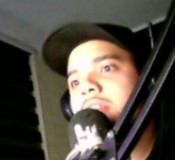
\includegraphics{grafico1.jpg}
%    \caption{Gráfico evolución del PIB. Fuente: Banco Central de Chile.}
%    \label{fig:my_label}
%\end{figure}

\newpage
\section*{Bibliografía}


\newpage
\section*{Anexos}




\end{document}